\documentclass[aspectratio=169]{beamer}
\usepackage[utf8]{inputenc}
\usepackage[english,russian]{babel}
%\usetheme{Madrid}
\usepackage{graphicx}
\graphicspath{{pictures/}}
\date[15 июня 2020 г.]{15 июня 2020 г.}
\title{Электроника стенда по изучению сцинтилляционных кристаллов}
\author{Андреев А. А. \\
        Научный руководитель: к.т.н. Жуланов В. В.}
\institute{Новосибирский Государственный Университет}

\makeatletter

\setbeamertemplate{footline}
{
    \leavevmode%
    \hbox{%
    \begin{beamercolorbox}[wd=.5\paperwidth,ht=2.25ex,dp=1ex,left]{title in head/foot}%
        \usebeamerfont{title in head/foot} A.A.Andreev@inp.nsk.su
    \end{beamercolorbox}%
    \begin{beamercolorbox}[wd=.5\paperwidth,ht=2.25ex,dp=1ex,right]{date in head/foot}%
        \usebeamerfont{date in head/foot}\insertshortdate{}\hspace*{2em}
        \insertframenumber{} / \inserttotalframenumber\hspace*{2ex} 
    \end{beamercolorbox}}%
    \vskip0pt%
}
\makeatother


\begin{document}

\begin{frame}
\titlepage
\end{frame}

\begin{frame}
\frametitle{Содержание}
    \begin{itemize}  
        \item Сцинтилляционные кристаллы
        \item Стенд по ислледованию сцинтилляционных кристаллов
        \item Задачи
        \item Операционная система
        \item Дизайн системы на кристалле
        \item Серверная часть
        \item Заключение
    \end{itemize}
\end{frame}

\begin{frame}
\frametitle{Сцинтилляционые кристаллы}
    Основные характеристики:
    \begin{itemize}  
        \item Конверсионная эффективность
        \item Технический выход
        \item Время высвечивания 
    \end{itemize}
\end{frame}

\begin{frame}
\frametitle{Установка стенда по исследованию сцинтилляционных кристаллов}
    \begin{columns}
        \begin{column}{0.3\textwidth}
            Блок-схема установки
        \end{column}
        \begin{column}{0.7\textwidth}
            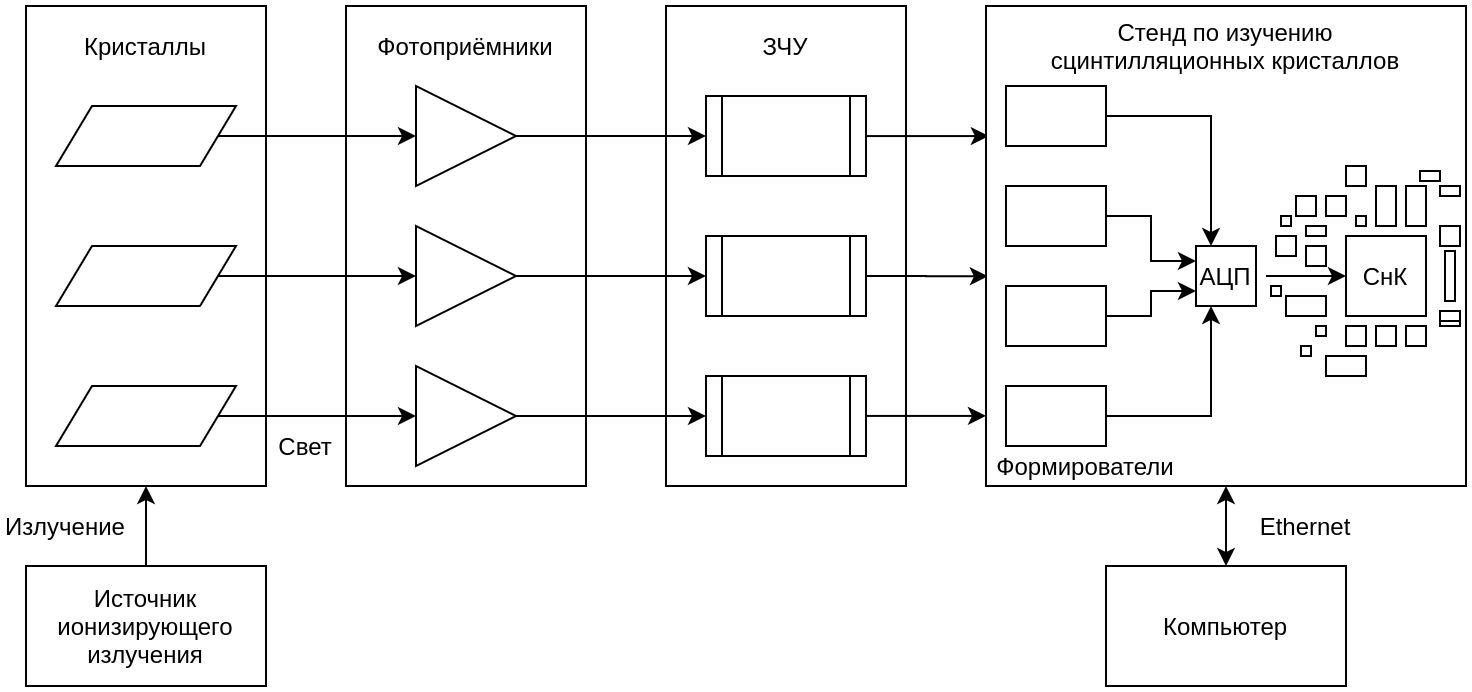
\includegraphics[width=\textwidth]{stand.jpg}
        \end{column}
    \end{columns}
\end{frame}

\begin{frame}
\frametitle{Стенд по исследованию сцинтилляционных кристаллов}
    \begin{columns}
        \begin{column}{0.4\textwidth}
            \begin{itemize}
                \item Набор формирователей 
                \item 4-х канальный 14-битный АЦП
                \item Система на кристалле Zynq 7000
            \end{itemize}
        \end{column}
        \begin{column}{0.6\textwidth}
            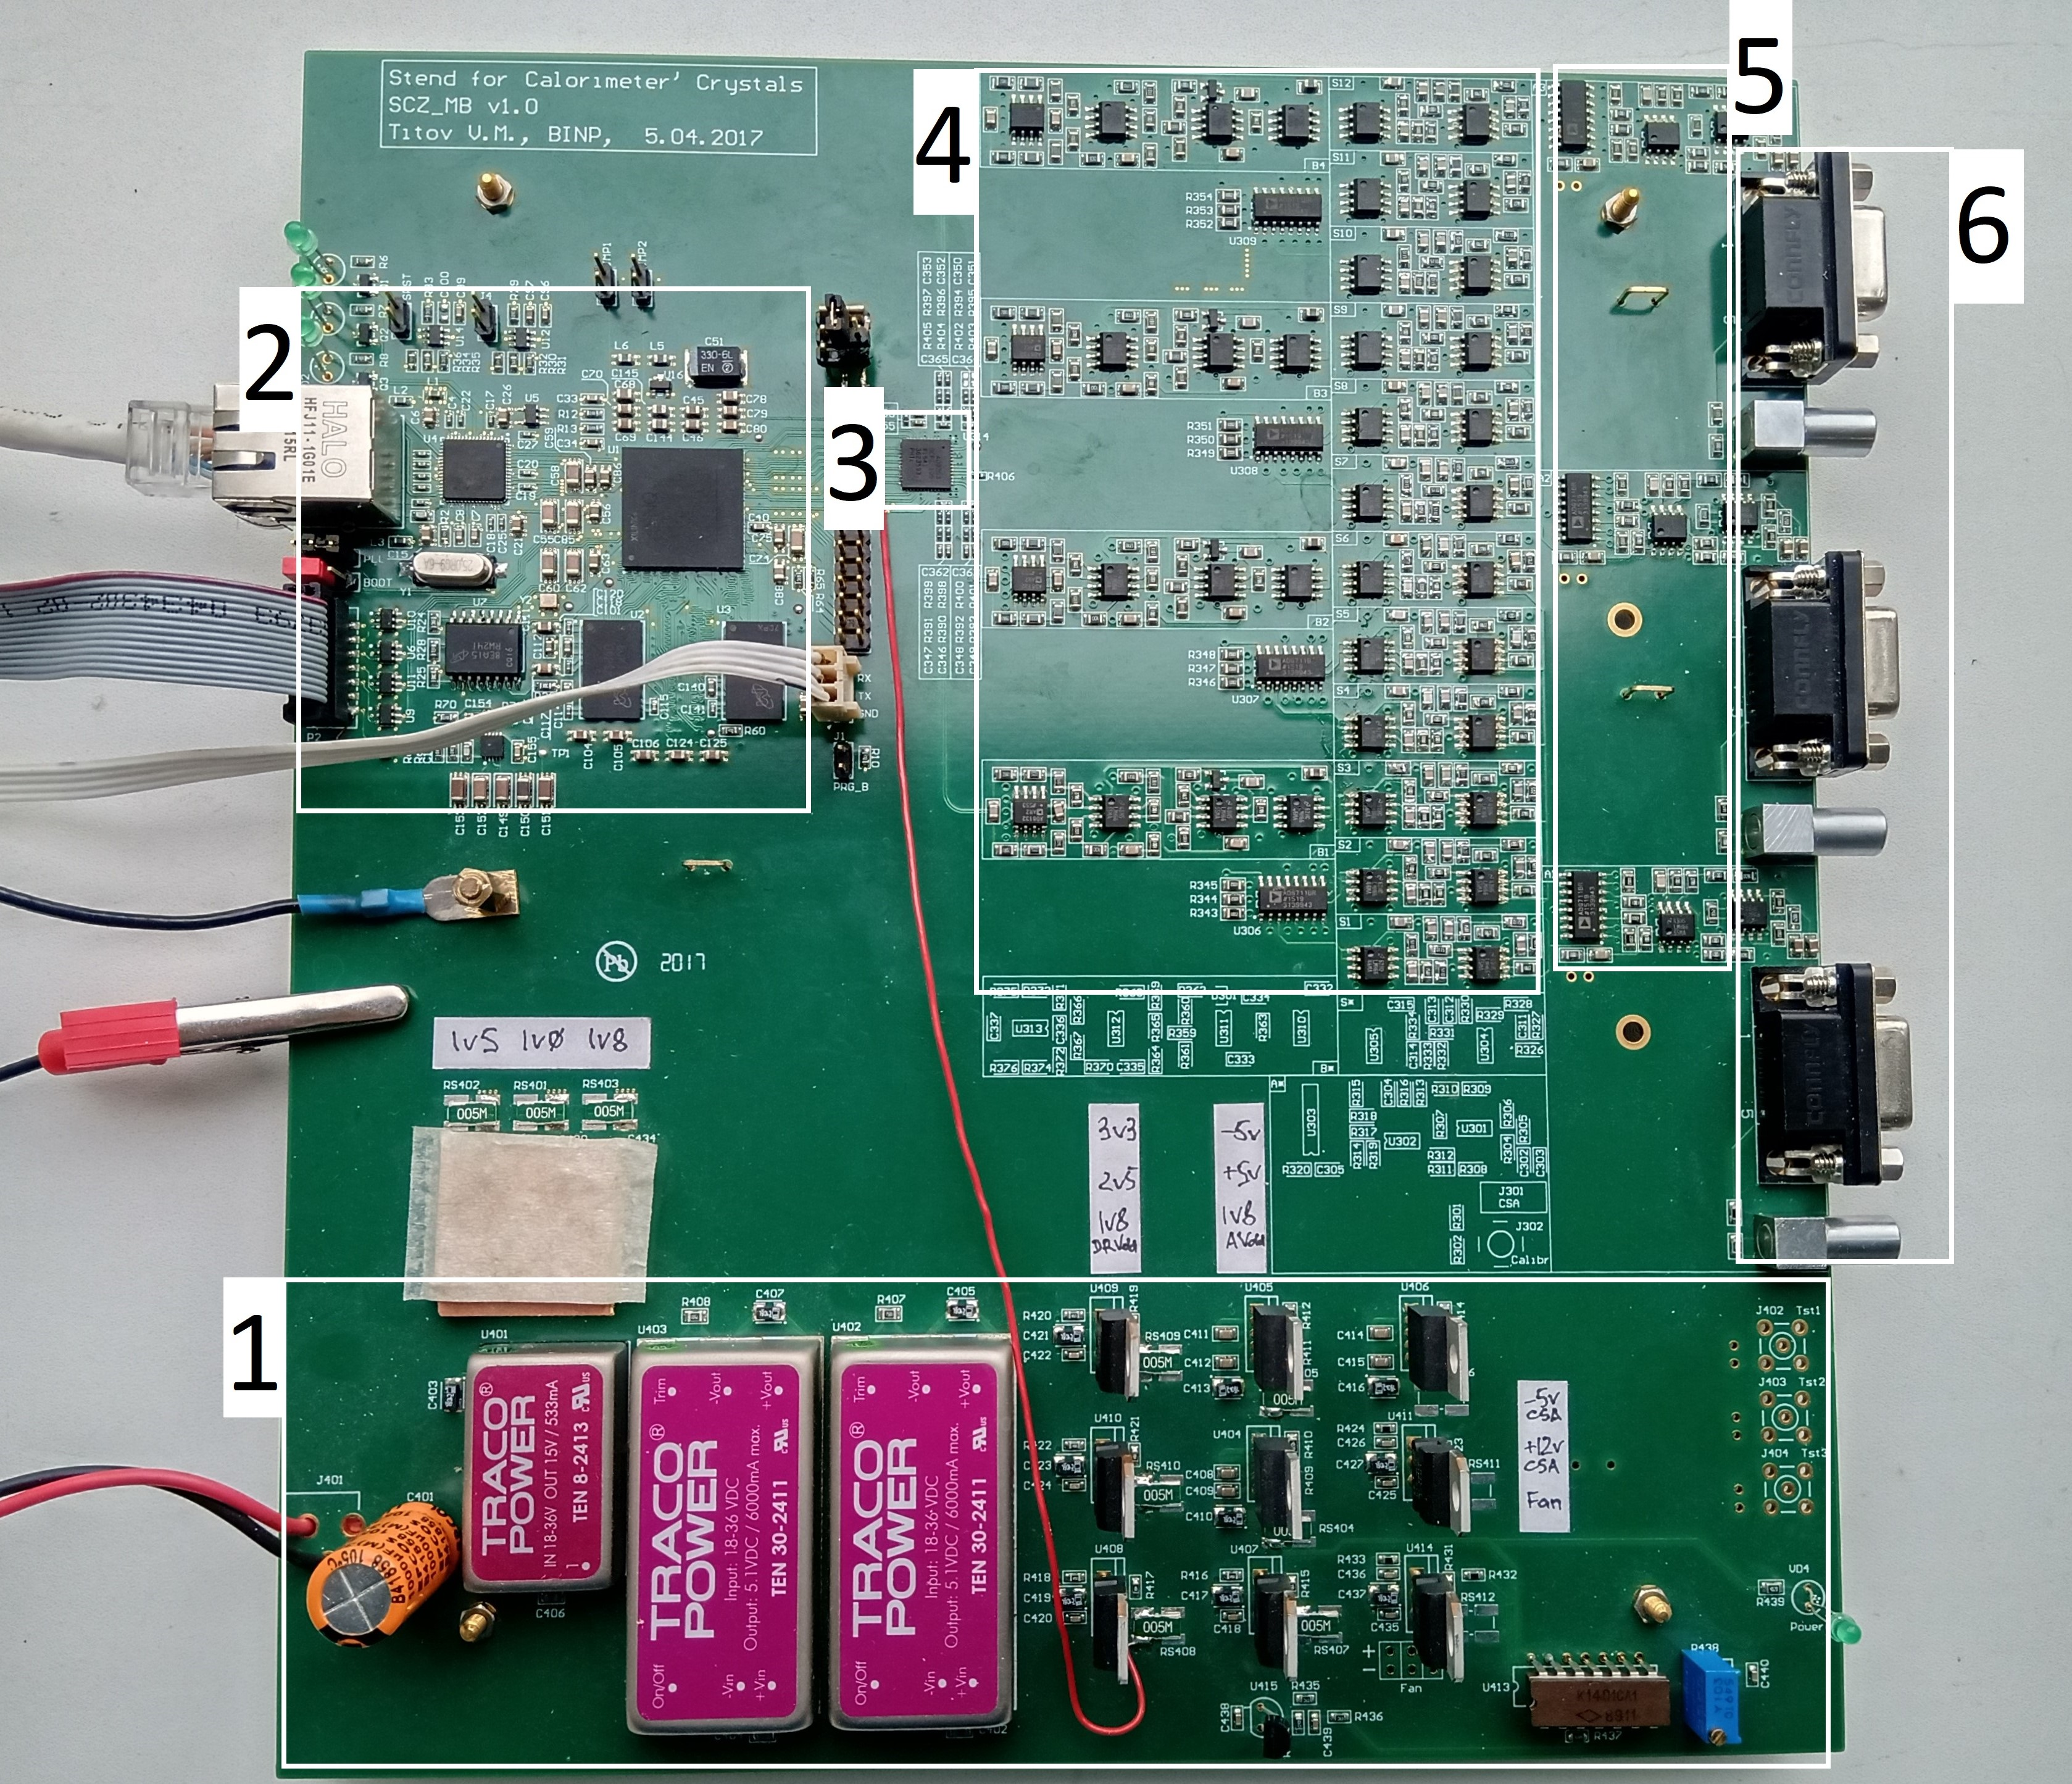
\includegraphics[width=\textwidth]{board.jpg}
        \end{column}
    \end{columns}
\end{frame}

\begin{frame}
\frametitle{Стенд по исследованию сцинтилляционных кристаллов}
    \begin{columns}
        \begin{column}{0.7\textwidth}
        Система на кристалле Zynq-7000 XC7Z020 CLG400
            \begin{itemize}
                \item 2-х ядерный процессор Cortex-A9
                \item ПЛИС Artix-7
            \end{itemize}
        Аналогово-цифровой преобразователь AD9253
            \begin{itemize}
                \item 4-х канальный 14-битный
                \item 100 МГц
                \item Serial LVDS
            \end{itemize}
        \end{column}
        \begin{column}{0.3\textwidth}
            
\includegraphics[width=\textwidth]{Zynq.jpg}
            
\includegraphics[width=\textwidth]{Analog_devices.jpg}
        \end{column}
    \end{columns}
\end{frame}

\begin{frame}
\frametitle{Задачи}
    Цель: разработать программное обеспечение для системы на кристалле.\par
    Задача: разработать прошивку которая включает в себя следущие модули:
    \begin{itemize}
        \item дизайн программируемой логики; 
        \item образ операционной системы;
        \item серверная часть
    \end{itemize}
\end{frame}

\begin{frame}
\frametitle{Дизайн системы на кристалле}
    \begin{columns}
        \begin{column}{0.2\textwidth}
        Процессорная система
        \end{column}
        \begin{column}{0.8\textwidth}
            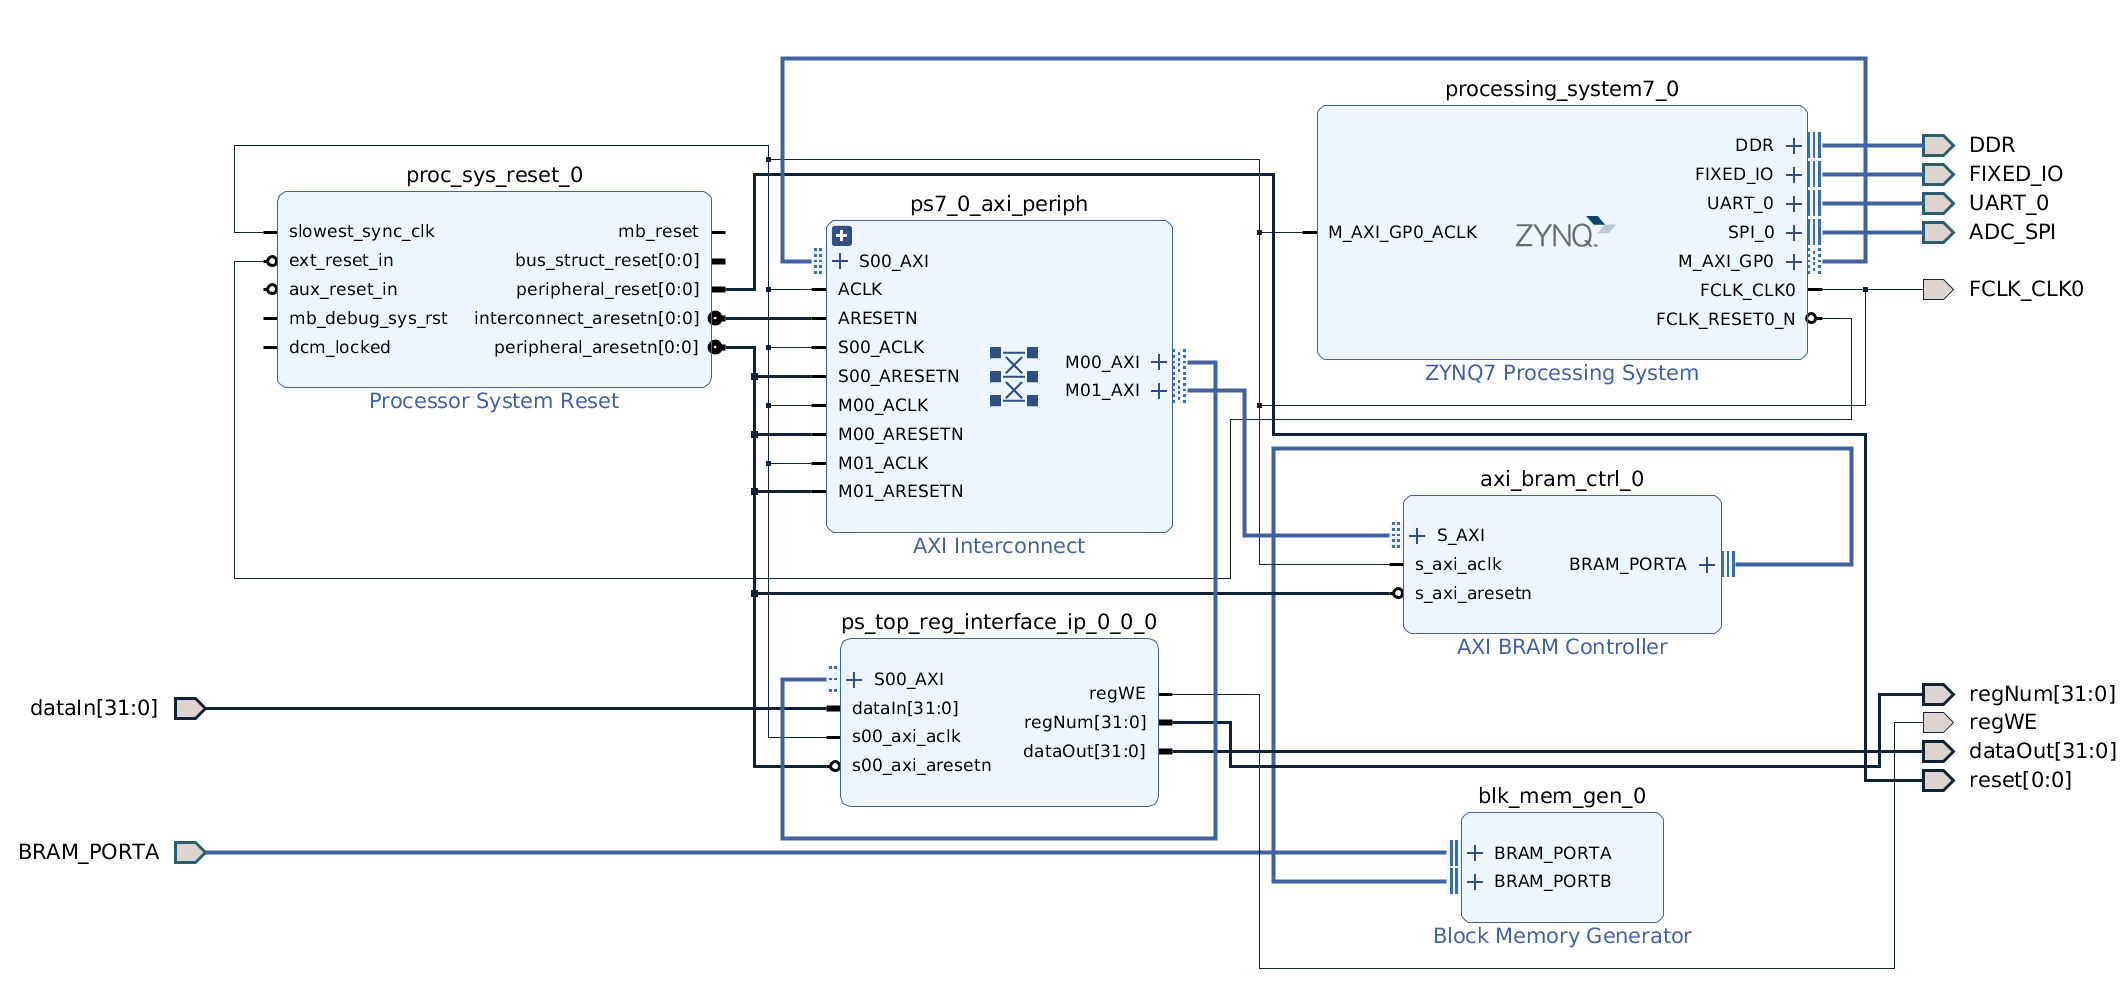
\includegraphics[width=\textwidth]{ps_top.jpg}
        \end{column}
    \end{columns}
\end{frame}

\begin{frame}
\frametitle{Дизайн системы на кристалле}
    \begin{columns}
        \begin{column}{0.4\textwidth}
        Программируемая логика
        \end{column}
        \begin{column}{0.5\textwidth}
            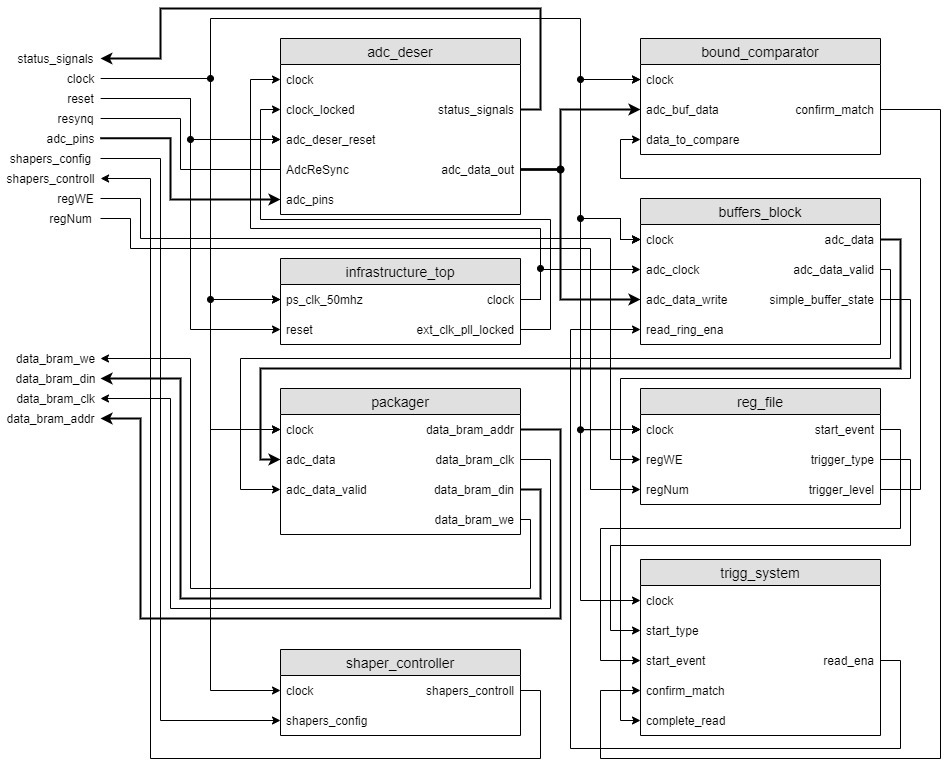
\includegraphics[width=\textwidth]{pl_top.jpg}
        \end{column}
    \end{columns}
\end{frame}

\begin{frame}
\frametitle{Операционная система}
Xilinx PetaLinux \\   
    \begin{columns}
        \begin{column}{0.8\textwidth}
            \begin{itemize}
                \item Ограничения:
                \begin{itemize}
                    \item автономность;
                    \item размер образа операционной системы
                \end{itemize}
                \item Требования:
                \begin{itemize}
                    \item настроенный сетевой интерфейс;
                    \item наличие необходимых пакетов в файловой системе
                \end{itemize}
            \end{itemize}
        \end{column}
        \begin{column}{0.2\textwidth}
            
\includegraphics[width=\textwidth]{Xilinx.jpg}
        \end{column}
    \end{columns}
\end{frame}

\begin{frame}
\frametitle{Серверная часть}
    \begin{columns}
        \begin{column}{0.25\textwidth}
            \begin{itemize}
                \item Сервер: Python, Django Framework
                \item Web-интерфейс: JavaScript, HTML, CSS
            \end{itemize}
        \end{column}
        \begin{column}{0.75\textwidth}
            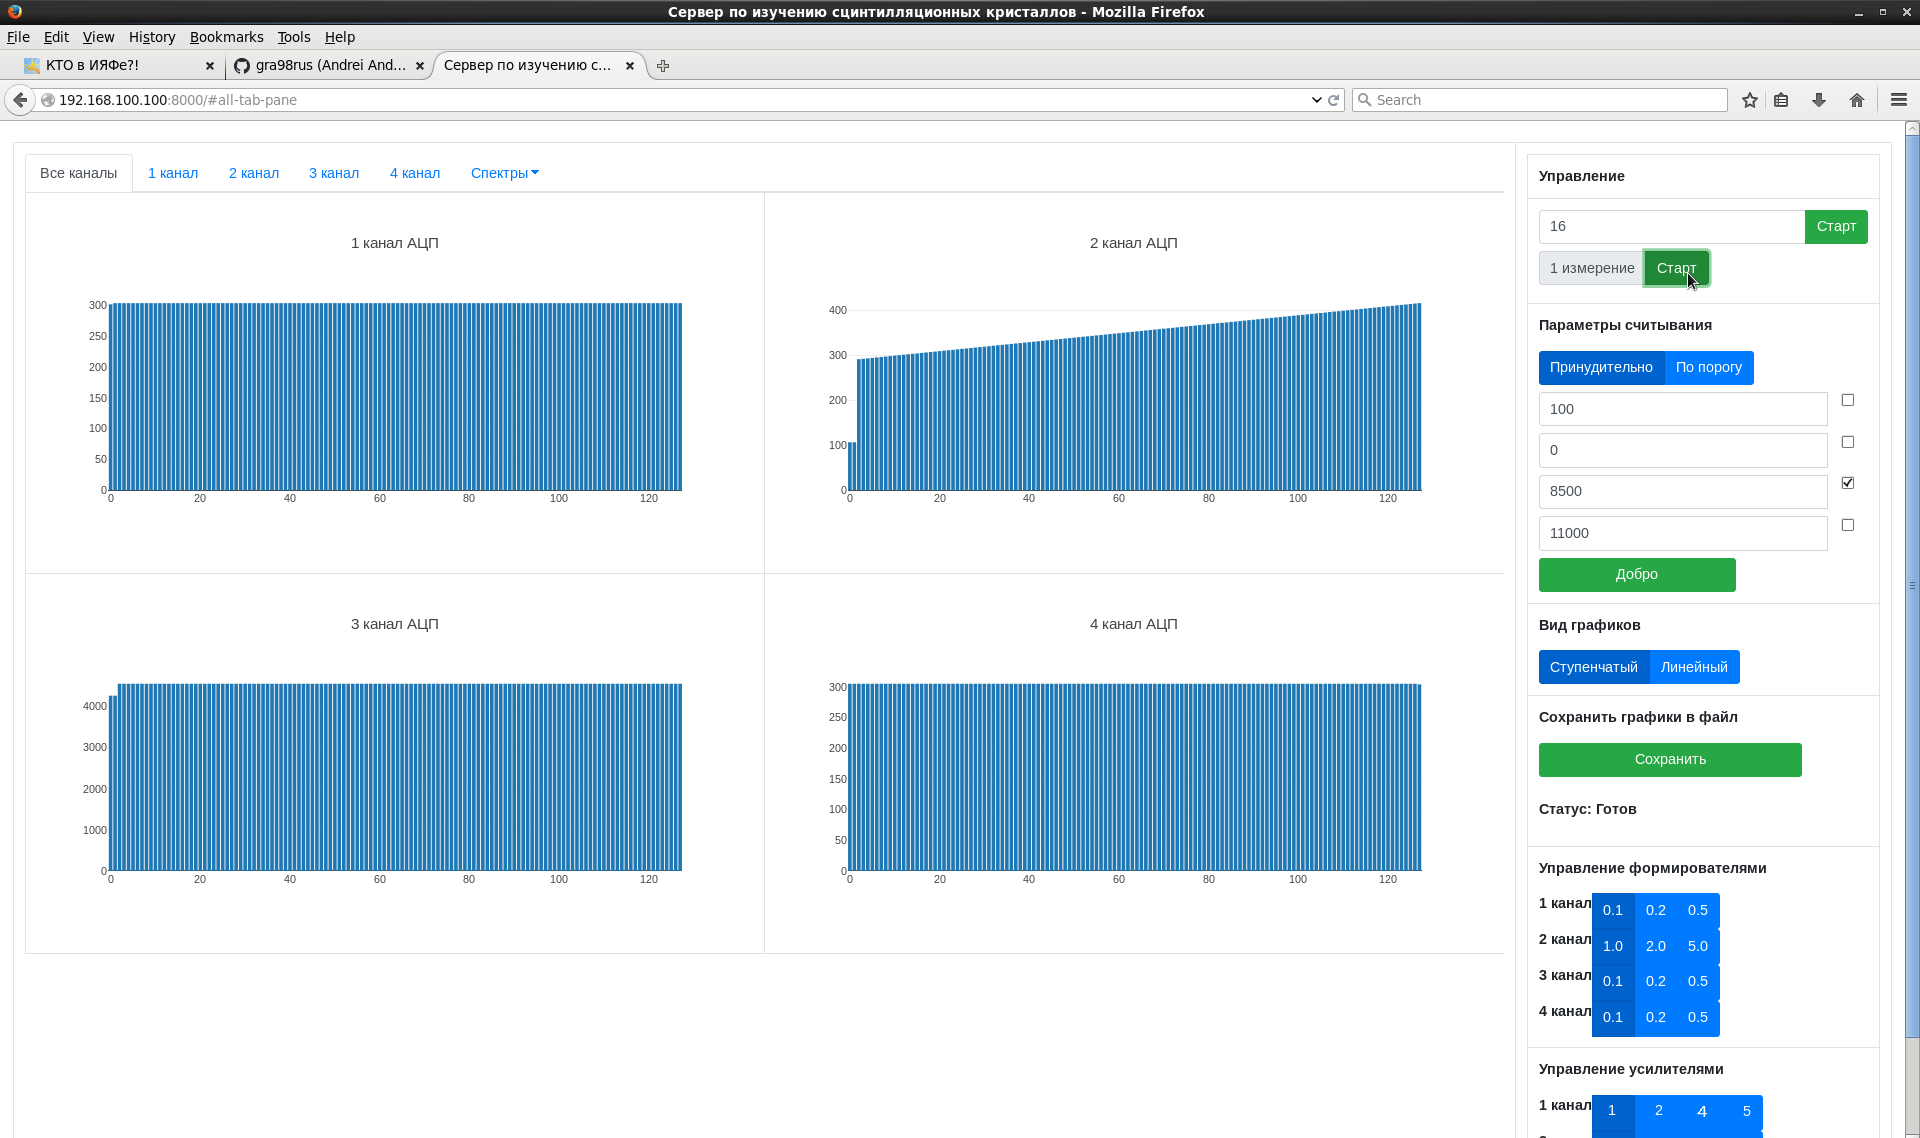
\includegraphics[width=\textwidth]{server.jpg}
        \end{column}
    \end{columns}
\end{frame}

\begin{frame}
\frametitle{Заключение}
    Выполнено:
    \begin{itemize}
        \item разработка прошивки системы на кристалле;
        \item сборка образа операционной системы;
        \item написание серверной части
    \end{itemize}
\end{frame}

\end{document}
